\documentclass{standalone}
\usepackage{tikz}
\usepackage{pgfplots}

\begin{document}
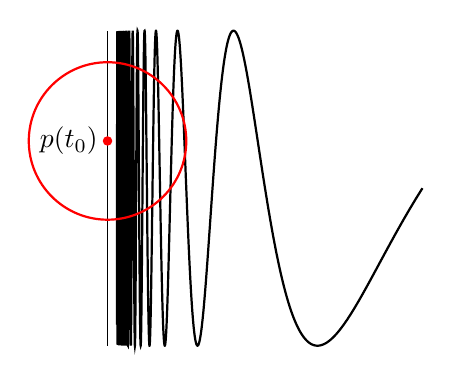
\begin{tikzpicture}[x=4cm, y=2cm]
\draw (0,-1) -- (0,1);
   % \draw[->] (0,-1) -- (0,1.1) node[above] {$\sin (1/x)$};
\draw[domain=0.03:1,samples=5000, smooth, thick] plot (\x, {sin((pi/\x)r)});

%  \filldraw[white] (0, 0) circle (31.7pt);
\draw[red, thick] (0, 0.3) circle (1cm);	
\filldraw[red] (0, 0.3) circle (1.5pt) node[black, left] {$p(t_0)$};
\end{tikzpicture}

\end{document}